Written by Anders Sjoqvist and Ulf Lundstrom, 2009
The main sources are: tinyKACTL, Beta and Wikipedia

\chapter{Matematicas}

\section{Ecuaciones}
\[ax^2+bx+c=0 \Rightarrow x = \frac{-b\pm\sqrt{b^2-4ac}}{2a}\]

Es extremos es dado por $x = -b/2a$.

\[\begin{aligned}ax+by=e\\cx+dy=f\end{aligned}
\Rightarrow
\begin{aligned}x=\dfrac{ed-bf}{ad-bc}\\y=\dfrac{af-ec}{ad-bc}\end{aligned}\]

En general dado un sistema $Ax = b$, la solucion de una variable $x_i$ es dada por
\[x_i = \frac{\det A_i'}{\det A} \]
donde $A_i'$ es $A$ con la $i$-esima columna remplazada por $b$.

\section{Recurrencias}
Si $a_n = c_1 a_{n-1} + \dots + c_k a_{n-k}$, y $r_1, \dots, r_k$ son raices distintas de $x^k + c_1 x^{k-1} + \dots + c_k$, hay $d_1, \dots, d_k$ tal que
\[a_n = d_1r_1^n + \dots + d_kr_k^n. \]
Raices diferentes $r$ se convierten en factores polinomiales, e.g. $a_n = (d_1n + d_2)r^n$.

\section{Trigonometria}
\begin{align*}
\sin(v+w)&{}=\sin v\cos w+\cos v\sin w\\
\cos(v+w)&{}=\cos v\cos w-\sin v\sin w\\
\end{align*}
\begin{align*}
\tan(v+w)&{}=\dfrac{\tan v+\tan w}{1-\tan v\tan w}\\
\sin v+\sin w&{}=2\sin\dfrac{v+w}{2}\cos\dfrac{v-w}{2}\\
\cos v+\cos w&{}=2\cos\dfrac{v+w}{2}\cos\dfrac{v-w}{2}
\end{align*}
\[ (V+W)\tan(v-w)/2{}=(V-W)\tan(v+w)/2 \]
donde $V, W$ son longitudes de angulos de lados opuestos $v, w$.
\begin{align*}
	a\cos x+b\sin x&=r\cos(x-\phi)\\
	a\sin x+b\cos x&=r\sin(x+\phi)
\end{align*}
donde $r=\sqrt{a^2+b^2}, \phi=\operatorname{atan2}(b,a)$.

\section{Geometria}

\subsection{Triangles}
Longitudes de los lados: $a,b,c$\\
Semiperimetro: $p=\dfrac{a+b+c}{2}$\\
Area: $A=\sqrt{p(p-a)(p-b)(p-c)}$\\
Circumradio: $R=\dfrac{abc}{4A}$\\
Inradio: $r=\dfrac{A}{p}$\\
Longitud de la mediana (Divide el triangulo en dos triangulos con el mismo area): $m_a=\tfrac{1}{2}\sqrt{2b^2+2c^2-a^2}$\\
Longitud de la bisectriz (Divide un angulo en dos): $s_a=\sqrt{bc\left[1-\left(\dfrac{a}{b+c}\right)^2\right]}$\\
Teorema del seno: $\dfrac{\sin\alpha}{a}=\dfrac{\sin\beta}{b}=\dfrac{\sin\gamma}{c}=\dfrac{1}{2R}$\\
Teorema del coseno: $a^2=b^2+c^2-2bc\cos\alpha$\\
Teorema de la tangente: $\dfrac{a+b}{a-b}=\dfrac{\tan\dfrac{\alpha+\beta}{2}}{\tan\dfrac{\alpha-\beta}{2}}$\\



\subsection{Cuadrilateros}

Con lados de longitud $a,b,c,d$, diagonales $e, f$, angulos de la diagonal $\theta$, area $A$ y "flujo magico" $F=b^2+d^2-a^2-c^2$:

$$4A = 2ef \cdot \sin\theta = F\tan\theta = \sqrt{4e^2f^2-F^2} $$

Para cuadrilateros ciclicos la suma de los angulos opuestos es $180^\circ$,
$ef = ac + bd$, y $A = \sqrt{(p-a)(p-b)(p-c)(p-d)}$.

\subsection{Coordenadas esfericas}
\begin{center}
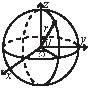
\includegraphics{content/math/sphericalCoordinates}
\end{center}
\[\begin{array}{cc}
x = r\sin\theta\cos\phi & r = \sqrt{x^2+y^2+z^2}\\
y = r\sin\theta\sin\phi & \theta = \textrm{arccos}(z/\sqrt{x^2+y^2+z^2})\\
z = r\cos\theta & \phi = \textrm{arctan}(y/x)
\end{array}\]

\section{Derivadas e Integrales}
\begin{align*}
	\dfrac{d}{dx}\arcsin x = \dfrac{1}{\sqrt{1-x^2}} &&& \dfrac{d}{dx}\arccos x = -\dfrac{1}{\sqrt{1-x^2}} \\
	\dfrac{d}{dx}\tan x = 1+\tan^2 x &&& \dfrac{d}{dx}\arctan x = \dfrac{1}{1+x^2} \\
	\int\tan ax = -\dfrac{\ln|\cos ax|}{a} &&& \int x\sin ax = \dfrac{\sin ax-ax \cos ax}{a^2} \\
	\int e^{-x^2} = \frac{\sqrt \pi}{2} \text{erf}(x) &&& \int xe^{ax}dx = \frac{e^{ax}}{a^2}(ax-1)
\end{align*}

Integracion por partes:
\[\int_a^bf(x)g(x)dx = [F(x)g(x)]_a^b-\int_a^bF(x)g'(x)dx\]

\section{Sumas}
\[ c^a + c^{a+1} + \dots + c^{b} = \frac{c^{b+1} - c^a}{c-1}, c \neq 1 \]
\begin{align*}
	1 + 2 + 3 + \dots + n &= \frac{n(n+1)}{2} \\
	1^2 + 2^2 + 3^2 + \dots + n^2 &= \frac{n(2n+1)(n+1)}{6} \\
	1^3 + 2^3 + 3^3 + \dots + n^3 &= \frac{n^2(n+1)^2}{4} \\
	1^4 + 2^4 + 3^4 + \dots + n^4 &= \frac{n(n+1)(2n+1)(3n^2 + 3n - 1)}{30} \\
\end{align*}

\section{Series}
$$e^x = 1+x+\frac{x^2}{2!}+\frac{x^3}{3!}+\dots,\,(-\infty<x<\infty)$$
$$\ln(1+x) = x-\frac{x^2}{2}+\frac{x^3}{3}-\frac{x^4}{4}+\dots,\,(-1<x\leq1)$$
$$\sqrt{1+x} = 1+\frac{x}{2}-\frac{x^2}{8}+\frac{2x^3}{32}-\frac{5x^4}{128}+\dots,\,(-1\leq x\leq1)$$
$$\sin x = x-\frac{x^3}{3!}+\frac{x^5}{5!}-\frac{x^7}{7!}+\dots,\,(-\infty<x<\infty)$$
$$\cos x = 1-\frac{x^2}{2!}+\frac{x^4}{4!}-\frac{x^6}{6!}+\dots,\,(-\infty<x<\infty)$$

\section{Probabilidad}
Sea $X$ una variable aleatoria con probabilidad $p_X(x)$ de tomar el valor $x$. Su esperanza es dada por $\mu=\mathbb{E}(X)=\sum_xxp_X(x)$ y varianza $\sigma^2=V(X)=\mathbb{E}(X^2)-(\mathbb{E}(X))^2=\sum_x(x-\mathbb{E}(X))^2p_X(x)$ donde $\sigma$ es la desviacion estandar. Si $X$ es una varibale contina la funcion de densidad es $f_X(x)$ y la suma de probabilidades con $p_X(x)$ es remplazada por la integral con $f_X(x)$.

La esperanza es lineal:
\[\mathbb{E}(aX+bY) = a\mathbb{E}(X)+b\mathbb{E}(Y)\]
Para $X$ e $Y$ independientes, \[V(aX+bY) = a^2V(X)+b^2V(Y).\]

\subsection{Distribuciones discretas}

\subsubsection{Binomial distribution}
El numero de aciertos $n$ independientes en experimentos si/no , donde cada acierto tiene una probabilidad de $p$ es $\textrm{Bin}(n,p),\,n=1,2,\dots,\, 0\leq p\leq1$.
\[p(k)=\binom{n}{k}p^k(1-p)^{n-k}\]
\[\mu = np,\,\sigma^2=np(1-p)\]
$\textrm{Bin}(n,p)$ es aproximadamente $\textrm{Po}(np)$ para pequeños $p$.

\subsubsection{DIstribucion del primer acierto (Geometrica)}
El numero de intentos necesarios hasta el primer acierto en experimentos de si/no, donde cada acierto tiene una probabilidad de $p$ es $\textrm{Fs}(p),\,0\leq p\leq1$.
\[p(k)=p(1-p)^{k-1},\,k=1,2,\dots\]
\[\mu = \frac1p,\,\sigma^2=\frac{1-p}{p^2}\]

\subsubsection{DIstribucion de Poisson}
El numero de eventos ocurridos en un tiempo determinado $t$ si esos eventos ocurren con una media de $\kappa$ independientemente del tiempo desde el ultimo suceso es $\textrm{Po}(\lambda),\,\lambda=t\kappa$.
\[p(k)=e^{-\lambda}\frac{\lambda^k}{k!}, k=0,1,2,\dots\]
\[\mu=\lambda,\,\sigma^2=\lambda\]

\subsection{Distribuciones continuas}

\subsubsection{Distribucion uniforma}
Si la funcion de densidad es constante entre $a$ y $b$ y es 0 fuera de  $\textrm{U}(a,b),\,a<b$.
\[f(x) = \left\{
\begin{array}{cl}
\frac{1}{b-a} & a<x<b\\
0 & \textrm{otherwise}
\end{array}\right.\]
\[\mu=\frac{a+b}{2},\,\sigma^2=\frac{(b-a)^2}{12}\]

\subsubsection{Distribucion exponencial}
El tiempo entre eventos en un proceso de Poisson es $\textrm{Exp}(\lambda),\,\lambda>0$.
\[f(x) = \left\{
\begin{array}{cl}
\lambda e^{-\lambda x} & x\geq0\\
0 & x<0
\end{array}\right.\]
\[\mu=\frac{1}{\lambda},\,\sigma^2=\frac{1}{\lambda^2}\]

\subsubsection{Distribucion normal}
Mucho de los sucesos aleatorios reales con media $\mu$ y varianza $\sigma^2$ son bien descritos por $\mathcal{N}(\mu,\sigma^2),\,\sigma>0$.
\[ f(x) = \frac{1}{\sqrt{2\pi\sigma^2}}e^{-\frac{(x-\mu)^2}{2\sigma^2}} \]
If $X_1 \sim \mathcal{N}(\mu_1,\sigma_1^2)$ and $X_2 \sim \mathcal{N}(\mu_2,\sigma_2^2)$ then
\[ aX_1 + bX_2 + c \sim \mathcal{N}(\mu_1+\mu_2+c,a^2\sigma_1^2+b^2\sigma_2^2) \]

\section{Cadenas de Markov}
Una \emph{Cadena de Markov} es un proceso aleatorio discreto con la propiedad de que el siguiente estado depende unicamente del estado actual.
Sean $X_1,X_2,\ldots$ unas secuencia de variables aleatorias generadas por un proceso de Markov.
Entonces hay una matriz de transicion $\mathbf{P} = (p_{ij})$, con $p_{ij} = \Pr(X_n = i | X_{n-1} = j)$,
y $\mathbf{p}^{(n)} = \mathbf P^n \mathbf p^{(0)}$ es la  distribucion de probabilidad para  $X_n$ (i.e., $p^{(n)}_i = \Pr(X_n = i)$),
donde $\mathbf{p}^{(0)}$ es la distribucion incial.

\subsubsection{Distribucion estacionaria}
$\mathbf{\pi}$ es una distribucion estacionaria si $\mathbf{\pi} = \mathbf{\pi P}$.
Si la cadena de Markov es \emph{irreducible} (es posible ir de cualquier estado a otro),
entonces $\pi_i = \frac{1}{\mathbb{E}(T_i)}$ donde $\mathbb{E}(T_i)$  es el tiempo esperado entre dos visitas en el estado $i$.
$\pi_j/\pi_i$ es el numero experado de visitas en el estado $j$ entre dos visitas del estado $i$.

Para un grafo conexo, no dirigido and no-bipartito, donde la la probabilidad de transicion es uniforme entre todos los vecinos, $\pi_i$ es proporcional al grado del nodo $i$.

\subsubsection{Ergodicidad}
Una cadena de Markov es \emph{ergodica} if the asymptotic si la distribucion asintotica es independiente del estado inicial de la distribucion.
Una cadena de Markov finita es ergodica si es irreducible y \emph{aperiodica} (i.e., el mcd de la longitud de los ciclos es 1).
$\lim_{k\rightarrow\infty}\mathbf{P}^k = \mathbf{1}\pi$.

\subsubsection{Absorvencia}
Una cadena de Markov es una A-cadena si los estados pueden ser particionados en dos conjuntos $\mathbf{A}$ y $\mathbf{G}$, tal que todos los estados en $\mathbf{A}$ son absorventes ($p_{ii}=1$), y tdos los estados en $\mathbf{G}$ acaban en un estado absorvente de$\mathbf{A}$.
La probabilidad para absorver en un estado $i\in\mathbf{A}$, donde el estado inicial es $j$, es $a_{ij} = p_{ij}+\sum_{k\in\mathbf{G}} a_{ik}p_{kj}$.
El tiempo esperado hasta la absorcion, donde el estado inicial es $i$, es $t_i = 1+\sum_{k\in\mathbf{G}}p_{ki}t_k$.
